%%%%%%weekly meeting template, prepared by Isaac Lee.  02/08/2017
\documentclass[11pt, a4paper]{article}
\usepackage{times}
\usepackage{ifthen}
\usepackage{amsmath}
\usepackage{amssymb}
\usepackage{graphicx}
\usepackage{setspace}

%%% page parameters
\oddsidemargin -0.5 cm
\evensidemargin -0.5 cm
\textwidth 15 cm
\topmargin -1.2 cm
\textheight 22 cm

\renewcommand{\baselinestretch}{1.4}\normalsize
\setlength{\parskip}{0pt}

\begin{document}
%%%mention the no, time, and venue of the meeting
\noindent Software Engineering Group Project PG 29 {\bf Client Meeting} on {\bf Tuesday 08/08/2017}.
\vspace*{10pt}
\begin{center}
\huge \bf Agenda
\end{center}

%%%first, nominate a chair for the meeting. We suggest that each member at least has one chance as the chair.
\section*{Chair: Ben}

\vspace*{10pt}

\section{Attendees}
\begin{itemize}
\item Chair: Ben
\item Facilitator: Pavi
\item TimeKeeper: Sean
\item Recorder: Isaac
\item Sammy
\item Huy Nguyen
\end{itemize}
%%%if some students cannot make the meeting due to some reasons, their names should appear here.

\section{Questions}
Questions for the client.

\subsection{General}
\begin{itemize}
\item What does the map look like, physical obstacles and lines?
\item No go zones, are they represented physically or just graphically on the map?
\item Is the starting location and orientation of the robot known?
\item How much of the map do we explore?
\item How is accuracy measured?
\item When can we access the robot?
\end{itemize}

\subsection{Technical}
\begin{itemize}
\item Wifi control detail?
\item How are the No Go Zones intended to be selected on the UI?
\end{itemize}

\section{System Overview}
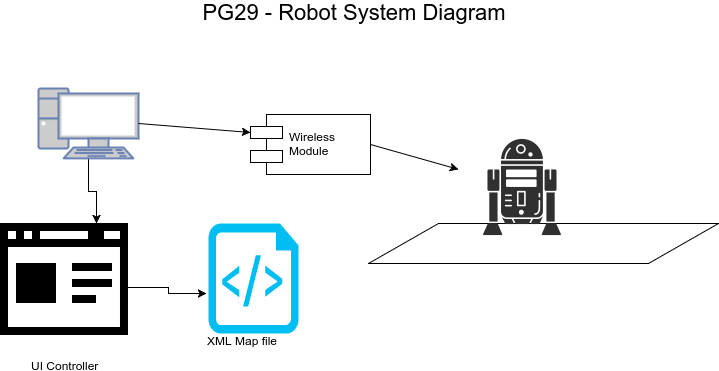
\includegraphics[width=\textwidth]{system-flowchart}

\section{Negotiation}
\begin{itemize}
	\item What milestones are most important?
	\item ....
\end{itemize}

\section{Next meeting}

\section{Other business}

\section {Close meeting}
%%%finally, specifies time of next meeting
\vspace*{10pt}


\end{document}
